\documentclass[a4paper,12pt]{article}
\setcounter{secnumdepth}{2}
\newcommand{\code}[1]{{\footnotesize{{\tt #1}}}}
\usepackage{natbib}
\usepackage{color}
\usepackage{graphicx}
\addtolength{\textwidth}{2cm} % a = -2b, where this is a and below is b
\addtolength{\hoffset}{-1cm}
\addtolength{\textheight}{2cm} % c = -d, where this is c and d is below
\addtolength{\voffset}{-2cm}
\begin{document}
\title{SnipSnip: GWAS for Poorly Tagged Data using Multiple SNPs}
\date{}
\author{}
\maketitle
\newpage
\tableofcontents
\newpage
\section{Introduction}
\label{introduction}

The SnipSnip program is the implementation of a GWAS method to detect causal variants using poorly tagged data by using multiple SNPs in low LD with the causal variant. Genome-wide association studies (GWAS) allow the detection of non-genotyped disease causing variants through the testing of nearby genotyped SNPs that are in strong linkage disequilibrium (LD) with the causal variant. This approach is naturally flawed when there are no genotyped SNPs in strong LD with the causal variant. There may, however, be several genotyped SNPs in weak LD with the causal variant that, when considered together, provide equivalent information. This observation provides the motivation for the popular (but computationally intensive) imputation-based approaches that are often used. 

SnipSnip is designed for the scenario where there are several genotyped SNPs in weak LD with a causal variant. Our approach proceeds by selecting, for each genotyped ``anchor'' SNP, a nearby genotyped ``partner'' SNP (chosen, on the basis of a specific algorithm we have developed, to be the optimal partner). These two SNPs are then used as predictors in a linear or logistic regression analysis, in order to generate a final significance test associated with the anchor SNP. 

SnipSnip is designed for use with {\bf unrelated individuals} either in a case-control analysis or a quantitative trait analysis. 

Our method, in some cases, potentially eliminates the need for more complex methods such as sequencing and imputation or haplotype analysis, and provides a useful additional test that may be used with existing GWAS data to identify genetic regions of interest. 

For an example application of SnipSnip see \citet{chen:etal:15}. 
\subsection{Program information and citation}
\label{information}

For details concerning the methodology of the SnipSnip GWAS, please see the accompanying manuscript \citet{howey:etal:14}. 

The program SnipSnip is written in C++ and executables are available for Linux and Windows from the download page, as well as the source code. 

Copyright, 2013 Richard Howey and Heather Cordell, GNU General Public License, version 3. 

%============ End of subsection "information"============


%================== End of section "introduction"==================

\section{Installation}
\label{installation}

Download an executable file from the home$\:$page for your system and off you go, or do the following. 
\begin{enumerate}

\item Download the code from the download page. 
\item Compile it by typing something like the following: \begin{verbatim}g++ -O3 *.cpp -o snipsnip \end{verbatim}

\item Start analysing your data with SnipSnip!\end{enumerate}

%================== End of section "installation"==================

\section{Using SnipSnip}
\label{using}
\subsection{Basic Usage}
\label{basic-usage}

The program SnipSnip takes a PLINK binary pedigree file as input. Basic usage of the program is given by typing: 
\begin{verbatim}
./snipsnip -o myresults.dat mydata.bed
\end{verbatim}

%============ End of subsection "basic-usage"============

\subsection{Options}
\label{options}

Typing \code{snipsnip} with no options will output usage details: 
\begin{verbatim}
SnipSnip: Imputation without imputation, v1.1
---------------------------------------------
Copyright 2013 Richard Howey, GNU General Public License, v3
Institute of Genetic Medicine, Newcastle University

Usage:
  ./snipsnip [options] pedigree.bed 
 or ./snipsnip -pf parameterfile [pedigree.bed]

Options:
  -window-size n    -- fix window at n SNPS, n must be even
  -window-size-bp x -- size of window, x, in kB
  -start a          -- start analysis from SNP number a
  -start-end a b    -- start and end analysis from SNP numbers a to b
  -i file.bed       -- input binary pedigree file, file.bed
  -o results.dat    -- output results file, results.dat
  -log results.log  -- log filename, results.log
  -covar covars.dat -- covariate filename, covars.dat
  -covar-number no  -- covariate number, no
  -covar-name na    -- covariate name, na
  -linear           -- use linear regression
  -mqtv x           -- missing quantitive trait value for linear regression
  -dominant         -- use dominant correlation partner metric
  -recessive        -- use recessive correlation partner metric
  -lr               -- perform standard logistic(linear) regression tests
  -excsnp bp        -- exclude SNP(base pair bp) as partner
  -so               -- suppress output to screen

Default Options in Effect:
  -window-size 10
  -o snipsnipResults.dat

\end{verbatim}

%============ End of subsection "options"============

\subsection{Parameter file}
\label{parameterfile}

A parameter file, \code{.pf}, may be used with SnipSnip instead of writing all of the options on the command line. To use a parameter file simply type: 
\begin{verbatim}
./snipsnip myparameters.pf
\end{verbatim}

The parameter file should be a text file with one option written on each line. For example, to perform an analysis with a SNP window of size 12, perform test for SNPs 100 to 200, include single SNP logistic regression results, with input file \code{mydata.bed} and output file \code{myresults.dat} the file \code{myparameters.pf} would be as follows: 
\begin{verbatim}
-window-size 12
-start-end 100 200
-lr
-i mydata.bed
-o myresults.dat
\end{verbatim}

It is also possible to add comments to the file provided that the ``-'' character is not used, and to comment out any options by placing another character in front of any ``-''. For example, the above parameter file could be edited as follows: 
\begin{verbatim}
I will use this window size
-window-size 12

Must remember to analysis other SNPs later
-start-end 100 200

Check single SNP logistic regression results also
-lr

This is my data
-i mydata.bed

Output the results here
-o myresults.dat

When I run lots of things I will suppress the output to screen 
#-so
\end{verbatim}

%============ End of subsection "parameterfile"============

\subsection{Input}
\label{input}

SnipSnip takes standard PLINK binary pedigree files, \code{.bed}, as input. This requires that the corresponding \code{.bim} and \code{.fam}, files are also available. A text PLINK pedigree file, \code{.ped}, with corresponding map file, \code{.map}, may be used to create a binary file using PLINK as follows: \begin{verbatim}
plink --noweb --file mydata --make-bed --out myfile
\end{verbatim}


This will create the binary pedigree file, \code{myfile.bed}, map file, \code{myfile.bim}, and family file, \code{myfile.fam} required for use with SnipSnip. 

%============ End of subsection "input"============

\subsection{Output}
\label{output}

The main results file is given by a text file where each row gives the results for each SNP. For example, using the default options gives the follows: 
\begin{verbatim}
SNP CHR ID BP PARTNER_ID PARTNER_BP CORRELATION SCORE FIT_STATUS CHISQ P
1 0 rs7112558 5569598 rs11038270 5572829 0.1875740 84.85855 Y 1.56046028 0.2115978
2 0 rs7123372 5569768 rs12786429 5570176 0.5597501 68.06836 Y 0.39244220 0.5310185
...
\end{verbatim}

The columns of the results file, which will differ depending on the chosen options, are as follows: 

{\begin{center}\begin{tabular}{ll}
Column  & Description\\
\hline
SNP  & The SNP number (of the anchor SNP) as it appears in file.\\
CHR  & Chromosome of the anchor SNP.\\
ID  & The name of the anchor SNP.\\
BP  & The base pair position of the anchor SNP.\\
PARTNER\_ID & The name of the partner SNP.\\
PARTNER\_BP & The base pair position of the partner SNP.\\
CORRELATION  & The correlation ( $r^2$ ) between the anchor SNP and partner SNP.\\
SCORE  & The score (0-100) between the anchor SNP and partner SNP. High scores are best.\\
FIT\_STATUS & A ``Y'' indicates that, yes, the model fitted with no problems. An ``N'' indicates that, no, the model did not fit, no doubt due to insufficient data in the cases and/or controls. A ``D'' indicates insufficient data in the cases and/or controls to even bother to try and fit the model.\\
CHISQ  & The $\chi^2$ test statistic with one degree of freedom from performing a likelihood ratio test comparing logistic regression models.\\
FSTAT  & The F test statistic with 1 and {\it number of subjects}-3 degrees of freedom from performing an F-test comparing linear regression models.\\
P  & The {\it p}-value for the test of association of the anchor SNP.\\
FIT\_STATUS\_LR & The fit status for single SNP logistic (or linear) regression at the anchor SNP.\\
CHISQ\_LR & The $\chi^2$ test statistic with one degree of freedom for single SNP logistic regression at the anchor SNP.\\
FSTAT\_LR & The F test statistic with 1 and {\it number of subjects}-3 degrees of freedom for single SNP linear regression at the anchor SNP.\\
P\_LR & The {\it p}-value for the test of association of the anchor SNP using single SNP logistic (or linear) regression.\\
\end{tabular}\end{center}}

%============ End of subsection "output"============


%================== End of section "using"==================

\section{SnipSnip GWAS}
\label{snipsnip-gwas}

A genome-wide association study (GWAS) can be performed using SnipSnip where each SNP is considered in turn as the {\it anchor} SNP and is tested for association with help from the {\it partner} SNP, see figure  \ref{anchor}. 
{\begin{figure}[ht]
{\begin{center}
{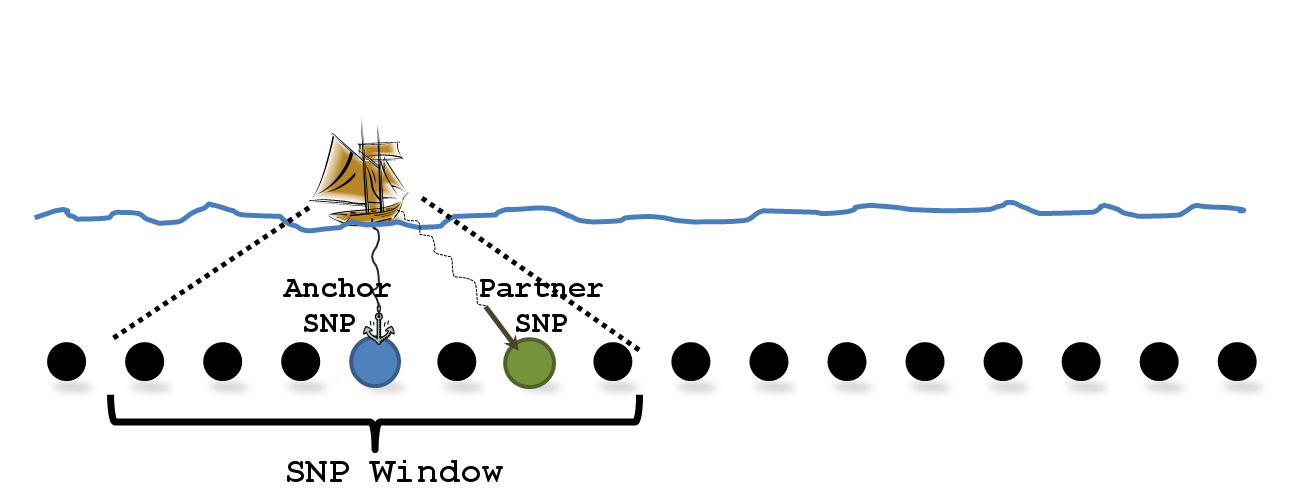
\includegraphics[width=400pt]{anchor.png}}
\caption{Diagram illustrating the anchor SNP and partner SNP with a SNP window of size 6.}
\label{anchor}
\end{center}}
\end{figure}
}
\subsection{Anchor SNP}
\label{anchor-snp}

The anchor SNP is simply the SNP that is being tested for association. 

%============ End of subsection "anchor-snp"============

\subsection{Partner SNP}
\label{partner-snp}

The partner SNP is chosen from a SNP window surrounding the anchor SNP and is the SNP with the ``best'' (not highest) LD with the anchor SNP. See  section \ref{metrics} for more infomation on how the partner SNP is chosen. 

%============ End of subsection "partner-snp"============

\subsection{AI Test}
\label{ai-test}

The artificial-imputation (AI) test is a likelihood ratio test comparing a logistic regression model with the partner SNP only against one with both the anchor SNP and partner SNP. The test produces a $\chi^2$ test statistic with one degree of freedom and tests the significance of the anchor SNP whilst conditioning for the partner SNP. An equivilent linear regression test is also possible. 

This is essentially a simple test and is only effective due to the manner in which the partner SNP is chosen. 

For more details concerning the methodology, please read the accompanying manuscript \citet{howey:etal:14}. 

%============ End of subsection "ai-test"============


%================== End of section "snipsnip-gwas"==================

\section{Partner SNP Metrics}
\label{metrics}

The partner SNP is chosen using the correlation between the anchor SNP and each potential partner SNP. The correlations are mapped to a score between 0 and 100, with 100 being the best. The SNP with the highest score is chosen as the partner SNP. The curves below (figure  \ref{metric-fig}) show the correlation-score maps assuming disease models which are multiplicative, dominant and recessive. 
{\begin{figure}[ht]
{\begin{center}
{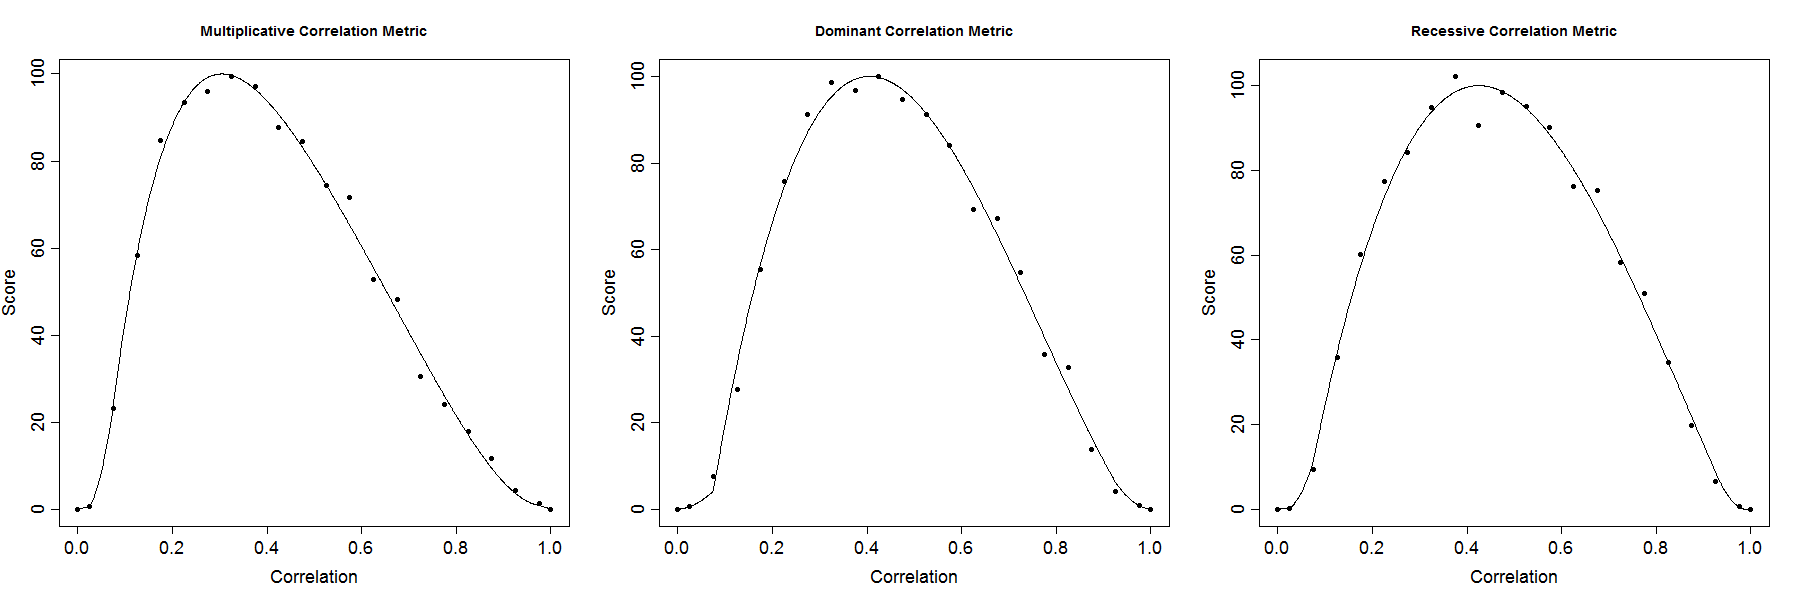
\includegraphics[width=400pt]{metrics.png}}
\caption{Plots of the partner SNP correlation metrics. Left to right, assuming a multiplicative, dominant and recessive causal variant model respectively.}
\label{metric-fig}
\end{center}}
\end{figure}
}

It is recommended that the default multiplicative causal variant model is used if the penetrances of any causal variants are unknown. The top 10 percent correlations are then in the interval [0.26, 0.36]. 

If it is known that the causal variant is dominant (recessive) then it should be beneficial to use the dominant (recessive) correlation metric using the \code{-dominant} (\code{-recessive}) option. (Note that the AI test still uses a multiplicative model and that this option only affects how the partner SNP is chosen.) 

Again, for more details concerning the methodology, please read the accompanying manuscript \citet{howey:etal:14}. 

%================== End of section "metrics"==================

\section{SNP Window Size}
\label{windowsize}

The window size of the SNP window used to pick the partner SNP for each anchor SNP is configurable using the \code{-window-size} option. It is only possible to set the SNP window size to an even number since the SNP window is in front and behind the anchor SNP. For example, to set the SNP window to size 12: 
\begin{verbatim}
./snipsnip -window-size 12 -o myresults.dat mydata.bed
\end{verbatim}

There is no ``correct'' window size, but 10 has proved in practise to be a good comprise between too small and too big, and is therfore set as the default. It is unlikely that a SNP window size of 20 or greater will be useful. If performing multiple GWASs with different SNP window sizes care should be exercised for multiple testing issues. 

It is also possible to set the SNP window using base pair position, so that any SNP within a certain base pair position distance of the anchor SNP is considered for the partner SNP. For example, to set the SNP window a base pair position size of 110,000: 
\begin{verbatim}
./snipsnip -window-size-bp 110000 -o myresults.dat mydata.bed
\end{verbatim}

However, it is recommended to use a fixed number of SNPs for the SNP window to increase the chances of picking a good partner SNP. 

Again, for more details concerning the methodology, please read the accompanying manuscript \citet{howey:etal:14}. 

%================== End of section "windowsize"==================

\section{Linear Regression}
\label{linear}

It is possible to use a quantitative trait for the phenotype instead of the case-control status. To do this use the \code{-linear} option. For example: 
\begin{verbatim}
./snipsnip -linear -o myresults.dat mydata.bed
\end{verbatim}

In this case the phenotype column in the \code{.fam} file should contain the phenotype of interest. The missing quantitative trait value is set by default to -9. This can be changed with the \code{-mqtv} option. For example, to set the missing quantitative trait value to 0: 
\begin{verbatim}
./snipsnip -linear -mqtv 0 -o myresults.dat mydata.bed
\end{verbatim}

When using linear regression the partner SNP is chosen in exactly the same manner as before and the same equivilent models are compared, but this time using an F-test. 

Again, for more details concerning the methodology, please read the accompanying manuscript \citet{howey:etal:14}. 

%================== End of section "linear"==================

\section{Covariates}
\label{covariates}

It is possible to perform the AI test with a set of covariates. To do this use the \code{-covar} option. For example: 
\begin{verbatim}
./snipsnip -covar covariates.dat -o myresults.dat mydata.bed
\end{verbatim}

The format of the covariate file is the same as PLINK covariate files. That is, a text file where the first column is the pedigree ID, the second column is the individual ID and the remaining columns are the covariate values, where a value of -9 denotes a missing value (this may be changed with the \code{-mqtv} option). For example, a covariate file with 3 covariates may look as follows: 
\begin{verbatim}
PEDID ID SMOKE ALCOHOL EX 
WXA_T1233 WXA_T120 0.0037 0.0033 0.0207
WXA_T1233 WXA_T121 -0.0019 0.022 0.0257
WXA_T1234 WXA_T987 0.0104 0.0096 -0.0154
...
\end{verbatim}

The header line may be present or not. The covariates may be chosen with the header names as follows: 
\begin{verbatim}
./snipsnip -covar covariates.dat -covar-name ALCOHOL,EX -o myresults.dat mydata.bed
\end{verbatim}

or 
\begin{verbatim}
./snipsnip -covar covariates.dat -covar-name ALCOHOL-EX -o myresults.dat mydata.bed
\end{verbatim}

to include all covariates between and including these two. Note that no spaces should be used between the chosen covariate values. The covariates may also be chosen by their numbers. So the above may be written: 
\begin{verbatim}
./snipsnip -covar covariates.dat -covar-number 2,3 -o myresults.dat mydata.bed
\end{verbatim}

or 
\begin{verbatim}
./snipsnip -covar covariates.dat -covar-number 2-3 -o myresults.dat mydata.bed
\end{verbatim}

%================== End of section "covariates"==================

\section{SnipSnip Examples}
\label{example}
\subsection{Basic example}
\label{ex-basic}

Using the example data given with the SnipSnip download, perform a basic SnipSnip analysis as follows: 
\begin{verbatim}
./snipsnip -o results-ExampleData.dat exampleData.bed
\end{verbatim}

In R type: 
\begin{verbatim}
exampleData<-read.table("results-ExampleData.dat", header=T)

plot(exampleData$BP/10^6, -log10(exampleData$P), main="SnipSnip Test",
 xlab=expression(bp~position~(Mb)), ylab=expression(-log[10](p-value)), ylim=c(0,15)) 
abline(h=8, lty=2)
\end{verbatim}

This will produce the following plot: 
{\begin{figure}[ht]
{\begin{center}
{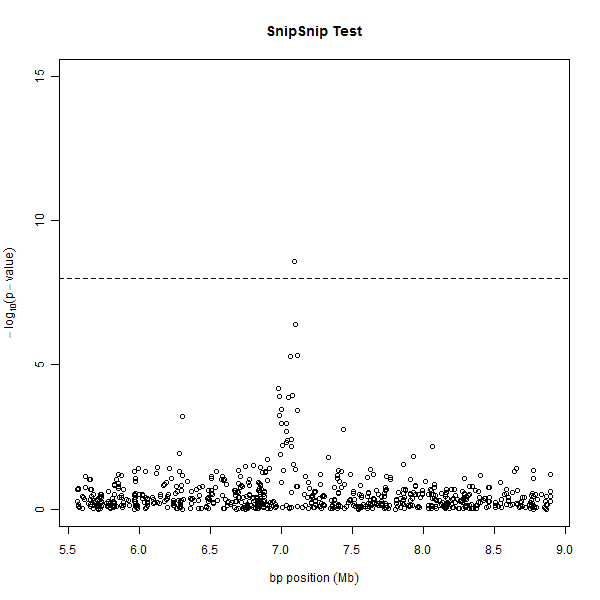
\includegraphics[width=200pt]{exampleSS.png}}
\caption{Manhattan plot of AI test results.}
\label{example-fig}
\end{center}}
\end{figure}
}

To also perform standard logistic regression use the \code{-lr} option as follows: 
\begin{verbatim}
./snipsnip -lr -o results-ExampleData-LR.dat exampleData.bed
\end{verbatim}

To plot the standard logistic regression test results type: 
\begin{verbatim}
exampleDataLR<-read.table("results-ExampleData-LR.dat", header=T)

plot(exampleDataLR$BP/10^6, -log10(exampleDataLR$P_LR), main="Standard Logistic Regression",
 xlab=expression(bp~position~(Mb)), ylab=expression(-log[10](p-value)), ylim=c(0,15)) 
abline(h=8, lty=2)

\end{verbatim}

This will produce the following plot: 
{\begin{figure}[ht]
{\begin{center}
{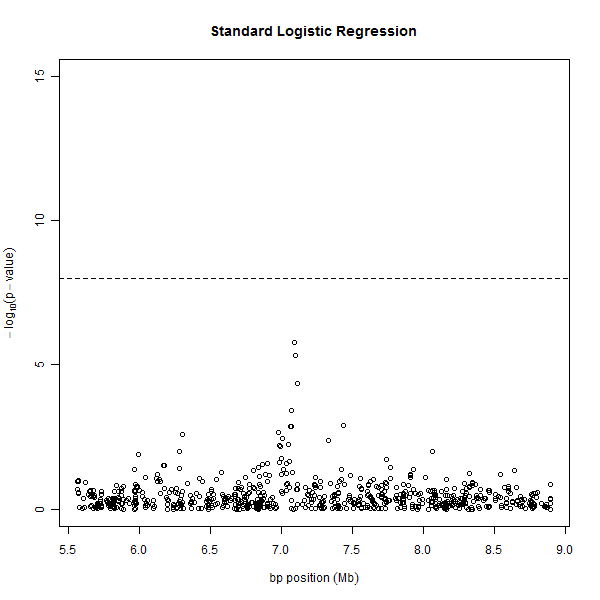
\includegraphics[width=200pt]{exampleSS_LR.png}}
\caption{Manhattan plot of standard logistic regression test results.}
\label{example-lr-fig}
\end{center}}
\end{figure}
}

%============ End of subsection "ex-basic"============

\subsection{X chromosome}
\label{X-chromosome}

SnipSnip does not do anything special with the analysis of SNPs on the X chromosome - the SNPs will be treated as if they were autosomal. (So females will end up with genotypes coded 0,1,2 and males will end up with genotypes coded 0,2). This has the potential to create false positives if you are dealing with a disease that has different prevalance in males and females; for this reason it is recommended to always include gender as a covariate if you are analysing X-chromosomal SNPs. See  section \ref{covariates} for details on handling covariates. 

If you have no other covariates to consider then it is possible to use the \code{.fam} file as the covariate file by choosing the sex column as the covariate as follows: 
\begin{verbatim}
./snipsnip -covar chromosome23.fam -covar-number 3 -o myresults-chr23.dat chromosome23.bed
\end{verbatim}

%============ End of subsection "X-chromosome"============


%================== End of section "example"==================

\bibliographystyle{genepi}
\bibliography{/home/nrajh/work-other/tex/biblio}
\end{document}